\documentclass[12pt,titlepage,a4paper]{article}
\usepackage[utf8]{inputenc}
\usepackage{amsmath}
\usepackage{amsfonts}
\usepackage{babel}
\usepackage{graphicx}
\usepackage{amssymb}
\usepackage{amsthm}
\usepackage{hyphenat}
\usepackage{caption}

\graphicspath{ {./images} }
\DeclareMathOperator*{\E}{\mathbb{E}}

\begin{document}

%===========================================================
\begin{titlepage}
\begin{center}

\textbf{\LARGE Spoken Dialog Systems}
%bei langen Titeln, die mehrere Zeilen benoetigen:
%\textbf{\LARGE Langer Titel der  ueber \medskip mehrere Zeilen laeuft}

\bigskip\bigskip
\textbf{Report}
%bei Masterarbeit:
%\textbf{Masterarbeit}

\bigskip\bigskip\bigskip
Written by

\bigskip
\textbf{Hanna Pankova}


\vfill
Faculty of Mathematics and Natural Sciences\\ 
Heinrich Heine University \\
D\"usseldorf

\bigskip
%Abgabedatum:
01 February 2022

\bigskip
Lecturer: Prof.\ Dr.\ Milica Ga\v{s}i\'{c}
%Wird der Schwerpunkt der Abschlussarbeit im Anwendungsfach gewaehlt:
%Betreuer: Prof.\ Dr.\ Vorname Nachname\\
%Zweitbetreuer: Prof.\ Dr.\ Vorname Nachname

\end{center}
\end{titlepage}

\thispagestyle{empty}\mbox{}
\setcounter{page}{0}

%===========================================================
\tableofcontents

\pagebreak
\section{Spoken Dialog Systems}
A spoken dialogue system is a computer system that enables human computer interaction where primary input is speech --- voice assistants (Siri, Alexa, etc.), chatbots, and etc. \par

A good spoken dialogue system is able to:
\begin{itemize}
     \item understand a user
     \item decide what to say back
     \item conduct a conversation beyond simple voice commands or question answering
\end{itemize}

Here only goal-oriented systems will be considered, where the scope of the conversation is usually limited to a specific domain with an ontology describing it.

System is usually split into separate modules with well-defined input and output, in each a machine learning algo\-rithm can be used (Figure \ref{fig:SDS-main}). Spoken language understanding (SLU) --- for detecting and encoding users' speech, Dialogue manage\-ment (DM) --- for tracking important imformation in the dialog and choosing correct answers, Spoken language gene\-ration (SLG) --- translating answers for a user into a speech. Modular approach has a downside of loosing information bet\-ween the modules, however ML approaches allow to consider a list of possible inputs with probabilities, and uncertainty gets propagated through the pipeline.

\begin{figure}[!h]
    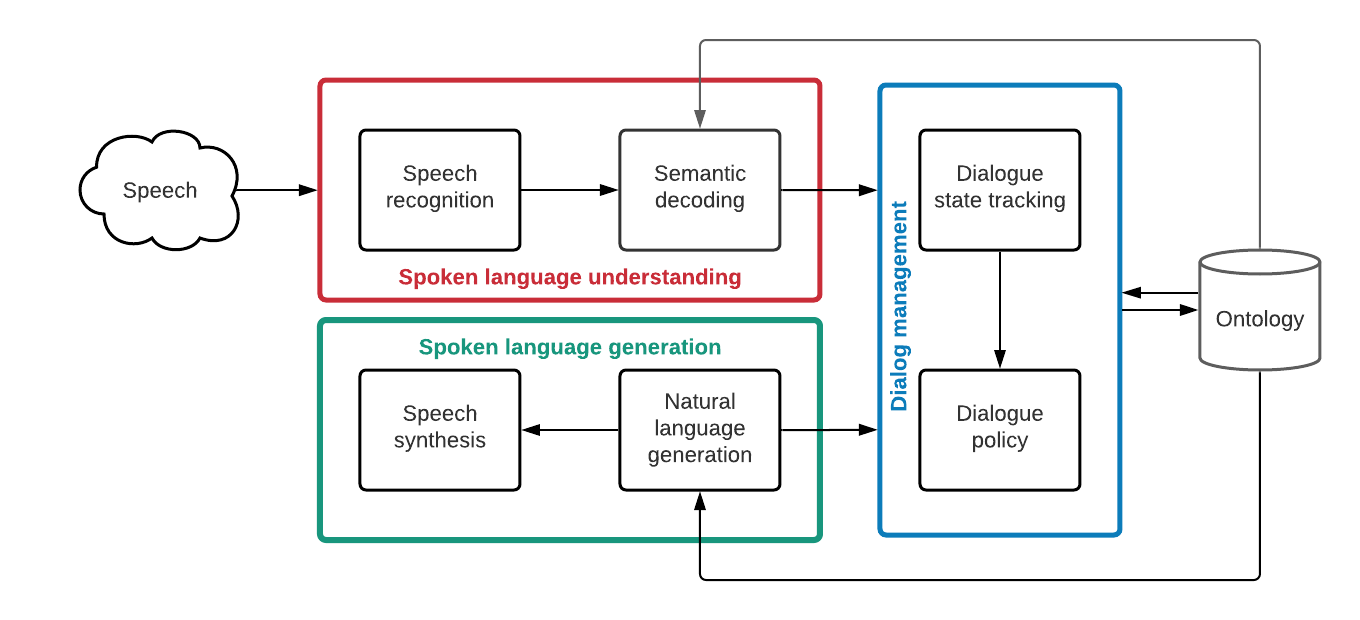
\includegraphics[width=\linewidth]{SDS-main.png}
    \caption{}
    \label{fig:SDS-main}
\end{figure}


\pagebreak
\section{Semantic Decoding}
Speech recogniser module of SLU translates speech into text and outputs a list of possible user utterances along with their probabilities (Figure \ref{fig:several}).

\begin{figure}[!h]
    \centering
    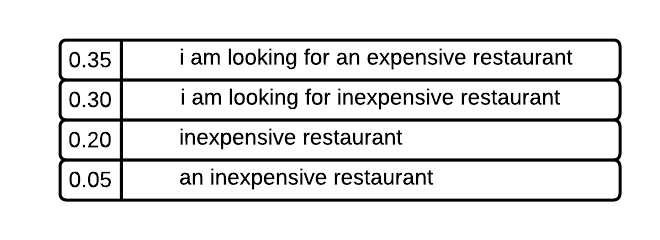
\includegraphics[width=0.65\linewidth]{uncertanty.png}
    \caption{}
    \label{fig:several}
\end{figure}
The task of a sematic decoder module is to get the meaning from them by translating utterances into a set of sematic concepts (dia\-log acts). Dialog act consists of: 

\begin{itemize}
    \item intent / dialog act type
    \item slot-value pairs
\end{itemize}

For instance a sentence ``Is there a cheap restaurant in the center?" translates into $inform(price=cheap,$ $area$ $=center)$, where $inform$ is an intent, $price$ is a slot with value $cheap$ and $area$ is a slot with value $center$.

\subsection{Models}
One approach would be to view semantic decoding as a classification task --- having a sepa\-rate probabi\-lity for each dialog act type and each slot-value pair.

\begin{figure}[h!]
    \centering
    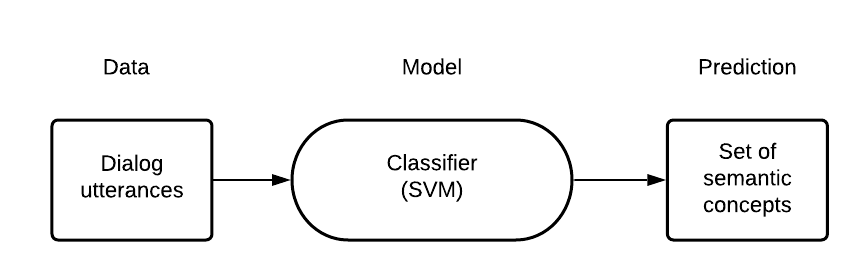
\includegraphics[width=0.8\linewidth]{training-2.png}
    \caption{}
\end{figure}

Utterance can be represented as a fixed-size vector, where only informa\-tion on which and how many words are there is preserved. To add positional information one can use an n-gram model. Delexicalisation clusters special terms as $area$ or $food-type$ with the help of ontology. Then several SVMs are trained to classify possible dialog acts (Figure \ref{fig:semantic-decoding-classification}).

\begin{figure}[h!]
    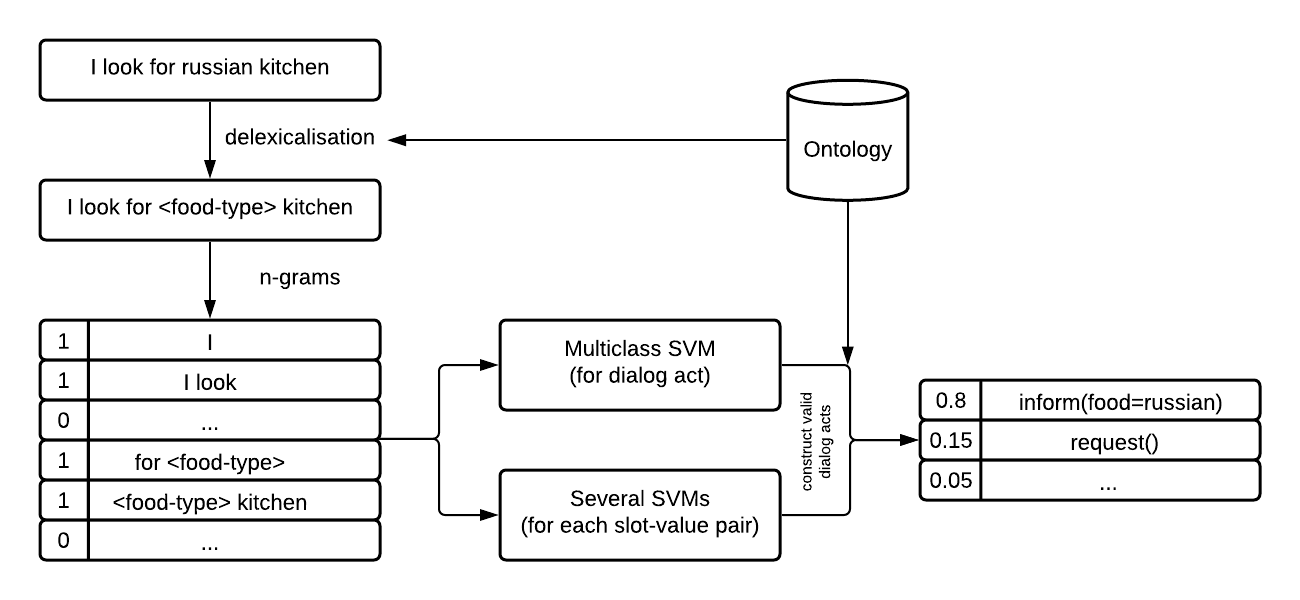
\includegraphics[width=0.998\textwidth]{semantic-decoding-classification.png}
    \caption{}
    \label{fig:semantic-decoding-classification}
\end{figure}

Another approach is to view it as a seq-to-seq task ---  translating an utterance into a sequence of tags, for ex.:

\begin{center}
    ``i want to fly from Minsk to Kiev round trip tomorrow" 
\end{center}

can be translated into the sequence of tags: 
\begin{center}
    ["O", "O", "O", "O", "O", "B-fromloc.city\_name", "O", "B-toloc.city\_name", "B-round\_trip", "I-round\_trip", "B-departure\_date"]
\end{center}
\begin{figure}[!h]
    \centering
    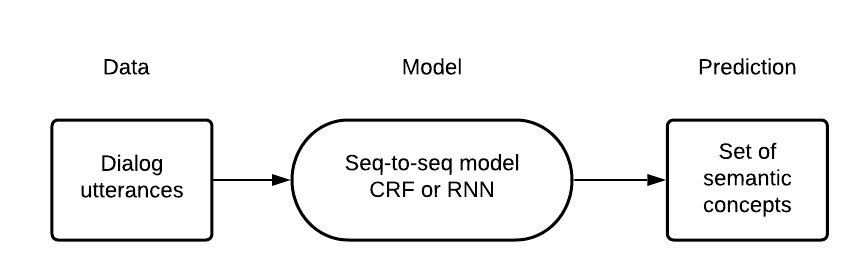
\includegraphics[width=0.91\linewidth]{training-2-2.png}
    \caption{}
    \label{fig:semantic-decoding-seq2seq}
\end{figure}

Model predicting a sequence of tags can be a simple RNN with two heads --- one for predicting the tags and another for predicting intent or conditional random fields (CRF) instead (Figure \ref{fig:semantic-decoding-seq2seq}).

\subsection{Evaluation for RNN model}

Having predictions from RNN the easiest mectric to calculate would be a f1-score on a slot level. One first collects slots from a predicted tags sequence:
\begin{center}
    input = [B-food-type\quad I\_food-type\quad O\quad B\_price-range\quad O] \\
    output = [(food-type, start=0, end=1), (price-range, start=3, end=3)]
\end{center}

Afterwards, having a set of true and predicted slots we can can calculate true posutives (TP), false positives (FP), false negatives (FN) on a slot level. Having these values one can calculate precision, recall and F1-score.

The other way to evaluate a model is to calculate TP, FP, FN for each tag, without converting them to slots. After there are two options on how to average the metrics: on a macro level (Equation \ref{eq:precision_macro}) and in a micro level (Equation \ref{eq:precision_micro}. Recall and F1-score are calculated analogically.

\begin{equation}
    Precision = \frac{1}{N_{slots}} \times \sum_{s \in slots}{s_{Precision}}
    \label{eq:precision_macro}
\end{equation}

\begin{equation}
    Precision = \frac{\sum_{s \in slots}{s_{TP}}}{\sum_{s \in slots}{s_{TP} + s_{FN}}}
    \label{eq:precision_micro}
\end{equation}

Macro average was much lower than a micro average (Table \ref{RNNMetrics}), because there can be a lot of classes with only few instances which were not predicted or predicted wrongly while there are not so many classes with a lot of instances, which are therefore predicted correctly, therefore without weight\-ning by the number of samples (micro level) one gets a lower average.

\begin{table}[!h]
    \centering
    \begin{tabular}{ | c | c | c | c | c |}
        \hline
                        & Precision & Recall & F1-score \\
        \hline
        accuracy        &           &        & 0.95 \\
        \hline
        marco average   & 0.48      & 0.46   & 0.45 \\
        \hline
        weighted average& 0.94      & 0.95   & 0.94 \\
        \hline
    \end{tabular}
    \caption{}
    \label{RNNMetrics}
\end{table}

Let's have a look on how the tags are recognised after training: 
\begin{center}
    \resizebox{\textwidth}{!}{
    \begin{tabular}{ c c c c c c c c c c c c c }
        & find & a & flight & from & tampa & to & montreal & by & way & of & new & york
        \\ 
        predicted & O & O & O & O & B-fromloc.city\_name & O & B-toloc.city\_name & O & O & O & B-fromloc.city\_name & I-fromloc.city\_name
        \\ 
        true & O & O & O & O & B-fromloc.city\_name & O & B-toloc.city\_name & O & O & O & B-stoploc.city\_name & I-stoploc.city\_name \\  
    \end{tabular}}
\end{center}

We can fix it by adding words ``with a stop in".
\begin{center}
    \resizebox{\textwidth}{!}{
    \begin{tabular}{ c c c c c c c c c c c c c c}
        & find & a & flight & from & tampa & to & montreal & with & a & stop & in & new & york
        \\ 
        predicted & O & O & O & O & B-fromloc.city\_name & O & B-toloc.city\_name & O & O & O & O & B-stoploc.city\_name & I-stoploc.city\_name  
    \end{tabular}}
\end{center}

Many instances where $state\_name$ was recognized as a $city\_name$: 
\begin{center}
    \resizebox{\textwidth}{!}{
    \begin{tabular}{ c c c c c c c c c c c}
        & please & find & a & flight & from & las & vegas & to & michigan
        \\ 
        predicted & O & O & O & O & O & B-fromloc.city\_name & I-fromloc.city\_name &  O & B-toloc.city\_name
        \\ 
        true & O & O & O & O & O & B-fromloc.city\_name & I-fromloc.city\_name &  O & B-toloc.state\_name \\  
    \end{tabular}}
\end{center}

$arrive\_time$ can be mistaken with $depart\_time$:
\begin{center}
    \scalebox{0.7}{
    \begin{tabular}{| c | c | c | c | c |}
        \hline
        Sentence & True & Predicted & Changes & New prediction\\
        \hline
        \hline
        i &O&O & i & O\\
        \hline
        would &O&O & would & O\\
        \hline
        like  &O&O & like & O\\
        \hline
        to &O& O & to & O\\
        \hline
        return &O& O & fly& O\\
        \hline
        from &O& O & around & B-depart\_time.time\_relative\\
        \hline
        chicago &B-fromloc.city\_name& B-fromloc.city\_name & 7 & B-depart\_time.time\\
        \hline
        around &B-depart\_time.time\_relative& B-depart\_time.time\_relative & in & O\\
        \hline
        7 &B-depart\_time.time& B-depart\_time.time & the & O\\
        \hline
        pm &I-depart\_time.time& I-arrive\_time.time & evening & B-depart\_time.period\_of\_day\\
        \hline
        to &O& O & from & O\\
        \hline
        kansas  &B-toloc.city\_name& B-toloc.city\_name & chicago & B-fromloc.city\_name\\
        \hline
        city &I-toloc.city\_name& I-toloc.city\_name & to & O \\
        \hline
        &&&kansas & B-toloc.city\_name\\
        \hline
        &&& city & I-toloc.city\_name\\
        \hline
    \end{tabular}}
\end{center}

We can fix wrongly recognized ``pm" by adding ``in the evening".
%===========================================================
\pagebreak
\section{Dialog state tracking}
Dialog state tracker os a part of dialog management module and remembers everything important that has happened in the dialog so far. Markov decision process (Figure \ref{MDP}) might be applied for tracking problem.

\begin{figure}[ht]
    \centering
    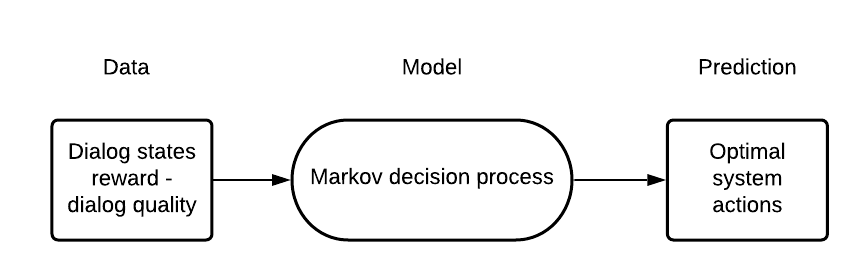
\includegraphics[width=0.8\linewidth]{training-state-tr-1.png}
    \caption{}
    \label{MDP}
\end{figure}

Process is represented as a dynamic Bayesian network (Figure \ref{Markov}) of: 
\begin{itemize}
    \item Dialog states --- current important information
    \item Actions --- what system does
    \item Rewards --- quality of the dialog so far
\end{itemize}

\begin{figure}[!htb]
    \minipage{0.38\textwidth}
      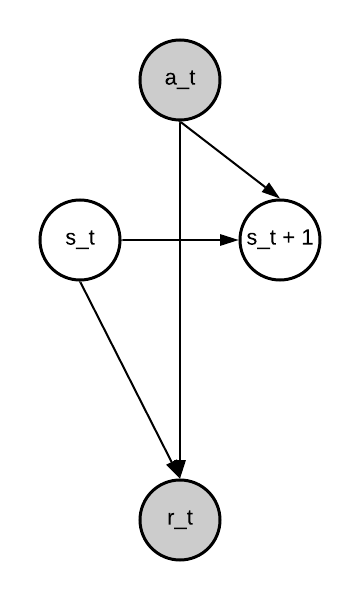
\includegraphics[width=\linewidth]{markov.png}
      \caption{}
      \label{Markov}
    \endminipage\hfill
    \minipage{0.38\textwidth}
      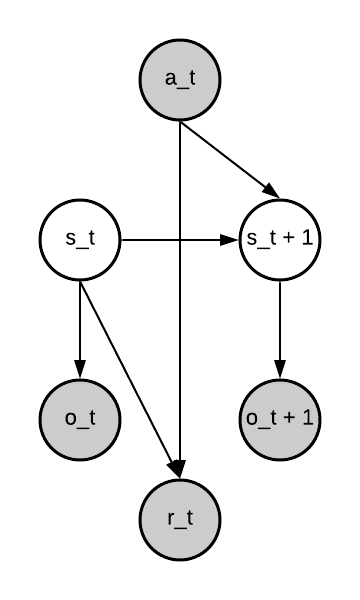
\includegraphics[width=\linewidth]{partial-markov.png}
      \caption{}
      \label{PartialMarkov}
    \endminipage
\end{figure}

One can assume that observed utteran\-ces are dependent on hidden states, then the process is called then partially observable Markov process (Figure \ref{PartialMarkov}).

Dialogue state is a set of distributions for the next components: 
\begin{itemize}
    \item Goal --- distribution over possible values (for each slot)
    \item Method --- distribution over possible methods
    \item Requested slots --- binary distribution (for each slot)
\end{itemize}

\subsection{Focus Tracker}

The simplest tracker assigns a single hypothesis for each slot at each turn, whereas a focus tracker accumulates evidence of a changing state over the course of the dialogue. It works in the following way: define for methods, goal components $c$ a quantity denoting that a slot / method is not present in turn $t$:

\begin{equation}
    \label{eqn:q_c_t}
    q_{c,t} := slu_{c,t}('none') = 1 - \sum_{v \in V_c \backslash \{'none'\}}slu_{c,t}(v)
\end{equation}

\noindent where $slu_c(v)$ --- a probability of a given slot value $v$ for goal $c$ be\-ing a correct one, $V_c$ --- all possible slot values.

Define $p_{c,t}(v)$ for each $v \in V_c \backslash \{'none'\}$ as: 
\begin{align}
    \label{eqn:p_c_t}
    p_{c,t}(v) &=slu_{c,t}(v) + q_{c,t} \cdot p_{c,t-1}(v) \\
    \label{eqn:p_c_0}
    p_{c,0}(v) &= slu_{c,0}(v) \\
    \label{eqn:p_c_t_none}
    p_{c,t}('none') &= 1 - \sum_{v \in V_c \backslash \{'none'\}}p_{c,t}(v)
\end{align}

For requestable slots $s$: 
\begin{align}
    \label{eqn:p_s_t}
    p_{s,t} &= slu_{s,t} + (1 - slu_{s, t})\cdot p_{s,t-1} \\
    \label{eqn:p_s_0}
    p_{s,0} &= slu_{s,0}
\end{align}

Let's prove that probabilities are well-defined, meaning that $0 \leq p_{c,t}(v) \leq 1$ $\forall v \in V_c, \forall t, \forall c$

\begin{proof}
    For goals(methods).
    Using method of mathematical induction for $t=0$: \\
    From (\ref{eqn:p_c_0}) since $0 \leq slu_{c,t}(v) \leq 1 \implies $

    \begin{equation}
        \begin{aligned}
            0 \leq &p_{c,0}(v) \leq 1 \\
            0 \leq &p_{c, 0}('none') \leq 1
        \end{aligned}
    \end{equation}

    \noindent Assuming that for $t = k-1$:

    \begin{equation}
        0 \leq p_{c,k-1}(v) \leq 1
    \end{equation} 

    \noindent Since

    \begin{equation}
        \begin{aligned}
            0 \leq slu_{c,k}(v) + slu_{c,k}('none') = 1 - \sum_{w \in V_{c} \backslash \{'none', v\}} slu_{c,k}(w) \leq 1
        \end{aligned}
    \end{equation}

    \noindent and $ slu_{c,k}(v) \geq 0 $,  $q_{c,k} \geq 0$, $p_{c,k-1}(v) \geq 0$
    then for $t=k$:

    \begin{equation}
        \begin{aligned}
            0 \leq p_{c, k}(v) \overset{
                \mathrm{\ref{eqn:p_c_t}}, 
                \mathrm{\ref{eqn:q_c_t}}
                }{=} slu_{c,k}(v) + q_{c,k} \cdot p_{c, k-1}(v) \leq 1
        \end{aligned}
    \end{equation}

    \noindent As $p_{c, t}('none') \leq 1$ from (\ref{eqn:p_c_t_none}), let's prove $p_{c, t}('none') \geq 0$.\\
    
    \noindent By method of mathematical induction assuming that for $t = k-1$ $p_{c, k-1}('none') \geq 0$ then for $t = k$:

    \begin{equation}
        \begin{aligned}
            p_{c,k}('none') 
            &\overset{
                \mathrm{\ref{eqn:p_c_t_none}},
                \mathrm{\ref{eqn:p_c_t}}, 
                \mathrm{\ref{eqn:q_c_t}}
                }{=} 1 - \sum_{v \in V_{c} \backslash \{'none'\}} \left[ slu_{c,k}(v) + q_{c,k} \cdot p_{c,k-1}(v) \right] \\ 
            &\overset{
                \mathrm{\ref{eqn:q_c_t}}
                }{=} slu_{c,k}('none') - \sum_{v \in V_{c} \backslash \{'none'\}} slu_{c,k}('none') \cdot p_{c,k-1}(v) \\ 
            &= slu_{c,k}('none')(1 - \sum_{v \in V_{c} \backslash \{'none'\}}p_{c, k-1}(v)) 
            \\
            &\overset{\sum_{V_c}p_{c, k-1}(v) = 1}{=} slu_{c,k}('none') \cdot p_{c, k-1}('none') \geq 0
        \end{aligned}
    \end{equation}

    For requestable slots. \\
    
    Assuming that for $t = k-1$:

    \begin{equation}
        0 \leq p_{s,k-1} \leq 1
    \end{equation}
    
    \noindent Since
    
    \begin{equation}
        0 \leq slu_{s,t} + (1 - slu_{s,t}) \leq 1
    \end{equation}

    \noindent Therefore

    \begin{equation}
        0 \leq p_{s,t} \overset{\ref{eqn:p_s_t}}{=} slu_{s,t} + (1 - slu_{s,t}) \cdot p_{s,t-1} \leq 1
    \end{equation}
\end{proof}

\subsection{Quality Evaluation}
For quality evaluation one can use either a fraction of turns where a top dialogue state hypothesis was correct (accuracy) or alternatively:
\begin{equation}
    L_2 = (1-p_i)^2 + \sum_{j \neq i} p_j^2
    \label{l2}
\end{equation}

\noindent
where $p$ is a hypothesised distribution, $i$ is an index of a true label. 

Focus tracker in comparison to the simplest tracker performs much better for goals (sometimes called informable slots) as they may change over time, for. ex. user may ask for another pricerange, location. However for request\-able slots its performance is not better as these slots usually should not change during the dialog, they are requested once, removed from the set, afterwards user can request next one. Similar for methods as the user usually "sets" by which method he will achieve the goal once (Table \ref{focus_tracker_results} and Table \ref{baseline_tracker_results}).

\begin{table}[ht]
    \centering
    \begin{tabular}{|c c c c|}
    \hline
                & Joint Goals & Requested & Method \\
    \hline
    Accuracy   & 0.73        & 0.92      & 0.68 \\ 
    L2         & 0.42        & 0.12      & 0.58 \\
    \hline
    \end{tabular}
    \caption{Focus Tracker}
    \label{focus_tracker_results}
\end{table}
\begin{table}[ht]
    \centering
    \begin{tabular}{|c c c c|}
    \hline
                & Joint Goals   & Requested & Method \\ 
    \hline
    Accuracy   & 0.57          & 0.91      & 0.68 \\ 
    L2         & 0.83          & 0.12      & 0.58  \\
    \hline
    \end{tabular}
    \caption{Simplest Tracker}
    \label{baseline_tracker_results}
\end{table}

\subsection{Interesting Question}
Assume user gives an exact same utterance in the first two turns of the dialog, what happens to a probability?

$slu(v) = slu_{c, 1}(v) = slu_{c,2}(v) \Rightarrow q_{c,1} = q_{c, 2} = q$ for $\forall c \forall v \in V_c $

\noindent Then
\begin{align*}
    &p_{c,2}(v) = slu_{c,2}(v) + q_c \cdot p_{c, 1}(v) 
    \\
    &p_{c,1}(v) = slu_{c,1}(v)
    \\
    &p_{c, 2}(v) = slu_{c,2}(v) + q_c \cdot p_{c, 1}(v) = slu(v)(1 + q_c) \geq p_{c,1}(v)
\end{align*}

\noindent $\Rightarrow$ probability of value $v$  for slot $c$ increases $p_{c,2}(v) \geq p_{c,1}(v) \forall v \in V_c $

\begin{align*}
    p_{c,2}('none') = 1 - \sum_{v \in V_{c} \backslash \{'none'\}} p_{c,2}(v) \leq 1 - \sum_{v \in V_{c} \backslash \{'none'\}} p_{c,1}(v)  = p_{c,1}('none')
\end{align*}

\noindent Probability of value $none$ decreases.
This is intuitive --- by a repetition user insists on some important information and agent becomes more confident in mentioned values and less in value $none$.

\subsection{Another update rule}
Define an update rule:
\begin{equation}
    p_{c,t}(v) = (1-q_{c,t})\cdot slu_{c,t}(v) + q_{c,t} \cdot p_{c,t-1}(v)
\end{equation}
Assume two turns of dialog happened and that for an informable slot $c$:
\begin{equation}
    \label{eqn:q_c_0_1}
    q_{c, 0} = 1
\end{equation}
and 
\begin{equation}
    \label{eqn:q_c_1}
    q_{c, 1} = slu_{c,1}(v) = 0.5
\end{equation}
for some $v$.

What happens to probability $p_{c,1}(v)$?

Since (\ref{eqn:q_c_0_1}) $\Rightarrow$ $p_c(v) = 0  \quad \forall v \in V_c\{'none'\} $, then: 
\begin{align*}
    p_{c,1}(v) = (1 - 0.5) \cdot 0.5 + 0 = 0.25
\end{align*}

As the slot was not in the first turn and then appeared in the second turn with probability 0.5, it is reasonable to assume that its probability might be not 0.5 (by previous update rule) but 0.25. 

In general, such update rule puts less weight on the new probabilities from current turn and more weight on the previous turn, which is also reasonable. 

\newpage

\section{Dialog optimisation as a reinforcement learn\-ing problem}
Apart from tracking a state of a dialog, the agent must learn to perform correct actions. This can be viewed as a reinforcement learning problem, where the agent is rewarded for performing correct actions and penalised for incorrect ones. Agent has a policy (its behaviour) that should be optimized, rewards from the environment, $V$-function (prediction of the future reward given current state $b$) and a model of environment.

$Q$-function is also defined to determines how good is it to take action $a$ in belief state $b$ and then follow a policy $\pi$. Having an optimal $Q$-function one can choose an optimal action.

\begin{equation}
    Q_{\pi}(b, a) = \E[R_t| b_t = b, a_t = a]
\end{equation}

The optimal value of Q is:
\begin{align}
    &V_{*}(b) = max_{\pi}V_{\pi}(b) \\
    &Q_{*}(b, a) = max_{\pi}Q_{\pi}(b, a) = \E[r_{t+1} + \gamma * V_{*}(b_{t+1})| b_t = b, a_t = a]
\end{align}

Optimal policy is: 
\begin{equation}
    \pi_{*}(b) = argmax_{a} Q_{*}(b, a)
\end{equation}


\subsection{Rewards}
Reward is a measure of success of the policy for the dialog, without reward one cannot learn an optimal policy. By optimizing reward value one opti\-mizes the policy. It is a metric for the algorithm's success.

\subsection{Allowed actions for execution}

For optimization one can restrict some actions to be executed as an agent should be not allowed to execute those actions which are clearly implausible. For example, after user requests a restaurant's address an agent should not say ``hello”. For that one can mask out with 0 those actions that are not allowed to be executed.

\subsection{Monte-Carlo policy}

Monte-Carlo control algorithm finds an optimal policy for a reinforcement learning problem.

It is a tabular approach, meaning that the belief state space is discretised into a grid. Following a random policy and $Q$-function one generates a dialog and rewards, which are iteratively used to update a $Q$-function and a policy afterwards. For updates the nearest state from the table is chosen (Figure \ref{fig:MCC}). 

\begin{figure}[!h]
    \centering
    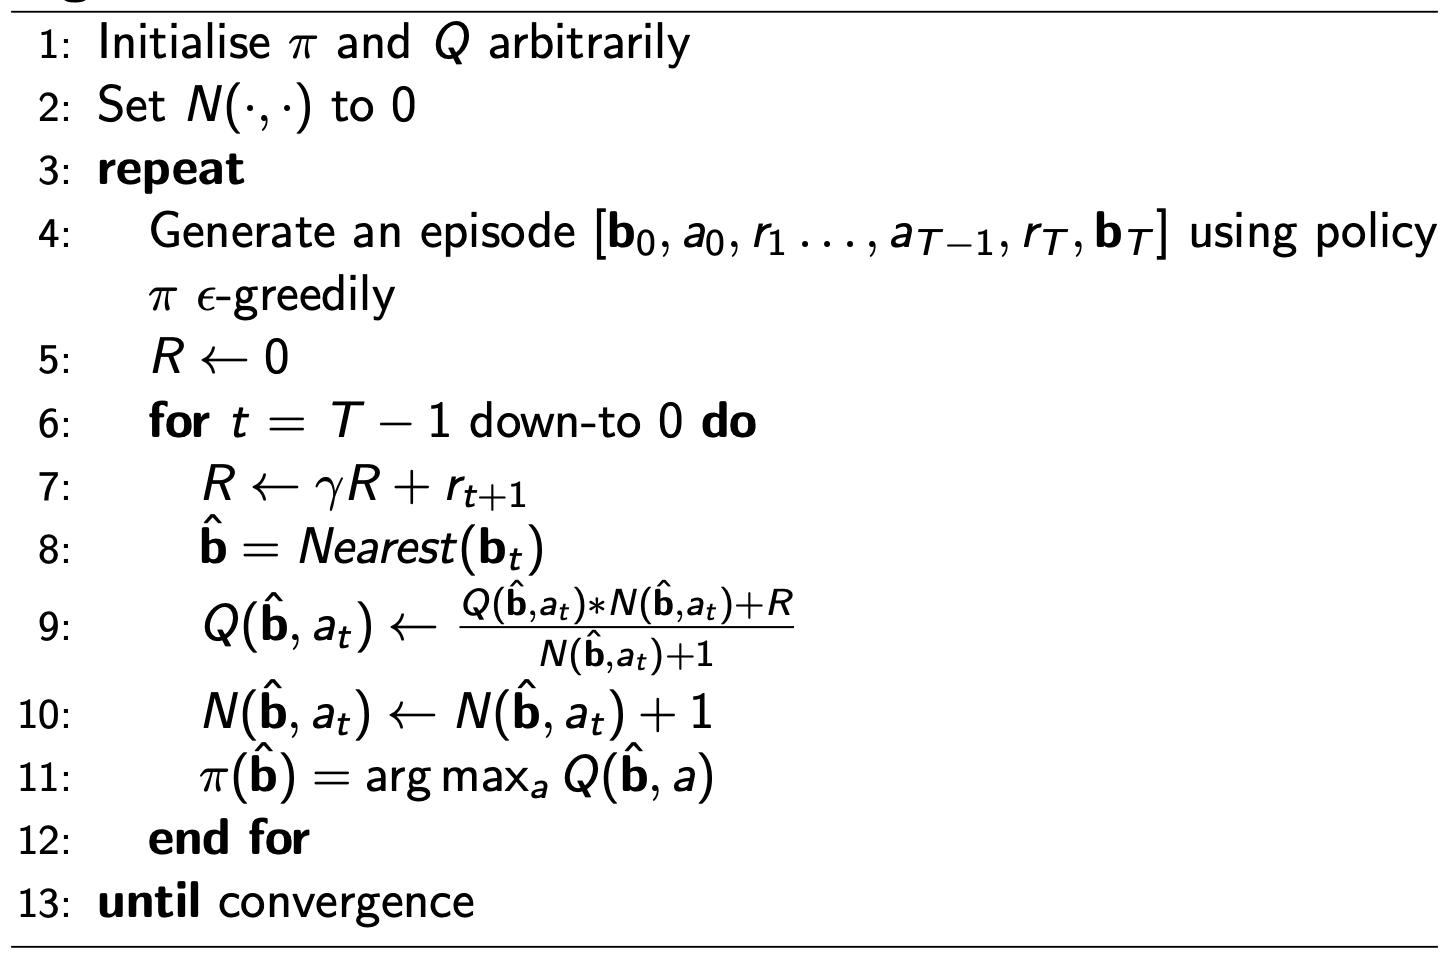
\includegraphics[width=10cm]{MCC.png}
    \caption{}
    \label{fig:MCC}
\end{figure}


\pagebreak


%===========================================================
\section{Deep Q-Learning}

%===========================================================
\subsection{Q-Network}
Instead of keeping Q-values in a table, one can approximate a Q-function with a neural network (Q-network). It takes a state of a dialog as input and outputs Q-values for each possible action. An optimal Q-network obeys the following Bellman optimality equation: 

\[ Q^*(s,a) = \E [r + \gamma max_{a^\prime}Q(s^\prime,a^\prime)] \] 

where $\gamma$ is a discount factor,  $r$ is an immediate reward and $\max_a Q(s',a)$ is the maximum Q-value of the next state. Bellman equation is used to update the Q-function iteratively:

\[Q_{i + 1} (s,a) \leftarrow \E[r + \gamma max_{a^\prime}Q_{i}(s^\prime,a^\prime)]\]

\subsection{Results}

In comparison to Monte-Carlo this approach is more efficient as it does not keep track of all the past states and remembers only the current one, because only Q-value of the current state is used for the next step update. Q-Network trains faster and better then a Monte-Carlo approach (TODO 96\% vs. 76\% Figures \ref{fig:ex}, \ref{fig:mc}). 

Two reasons for benefits of DQN over Monte-Caro are: experience replay and delayed Q-targets. For experience replay one stores tuples ${s, a, r, s^\prime}$ in the buffer, where $s^\prime$ is the following dialog state and samples batches from the it. Delayed targets allow to stabilize the network as we the target network’s parameters are not trained, but periodically synchronized with the main Q-network. Loss function:

\[\L = \E_{(s, a, r, s^\prime) \sim D} [(Q_{target}(r,s^\prime) - Q(s, a))^2]\]

where 

\[Q_{target}(r, s^\prime) = r + \gamma max_{a}Q_{target}(s^\prime,a)\]

Let's train a Q-network without experience replay. In this case reward was almost 3 times lower TODO (11.23 and 4.5 Figure \ref{fig:no-ex}, Table \ref{tab:replay-no-replay}). With increased variance the $Q$-network became more unstable.
\begin{table}[!h]
    \centering
    \begin{tabular}{||c c c c||} 
     \hline
      & Reward & Success & Turns \\ [0.5ex] 
     \hline\hline
     Experience replay & TODO 11.23 +- 0.97 & 93.00 +- 3.56 & 7.37 +- 0.53 \\ 
     \hline
     No experience replay & 4.50 +- 2.04 & 69.00 +- 6.45 & 9.30 +- 0.94 \\
     \hline
    \end{tabular}
    \caption{}
    \label{tab:replay-no-replay}
\end{table}

TODO change images
\begin{figure}[!htb]
    \minipage{0.32\textwidth}
      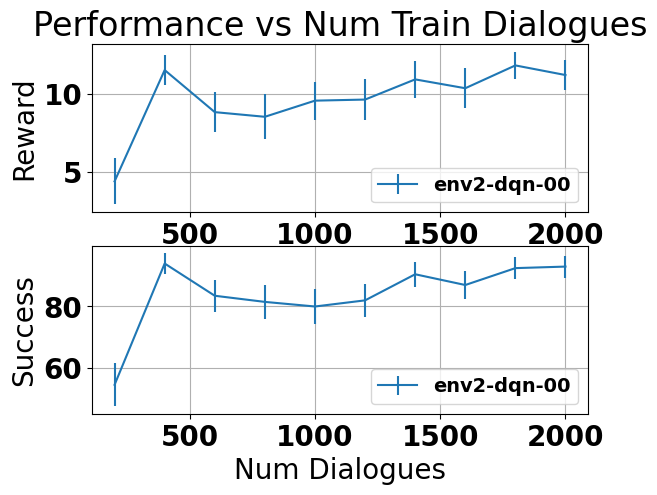
\includegraphics[width=\linewidth]{env2-CamRestaurants-experience.png}
      \caption{Experience Replay}
      \label{fig:ex}
      \endminipage\hfill
    \minipage{0.32\textwidth}
      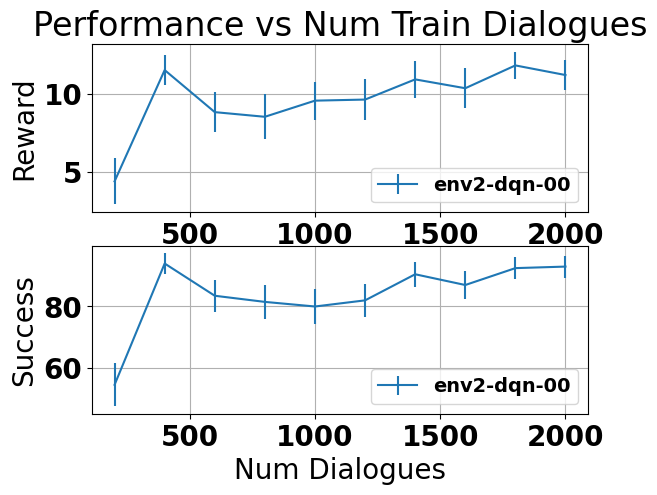
\includegraphics[width=\linewidth]{env2-CamRestaurants-experience.png}
      \caption{No Experience Replay}
      \label{fig:no-ex}
      \endminipage\hfill
    \minipage{0.32\textwidth}%
      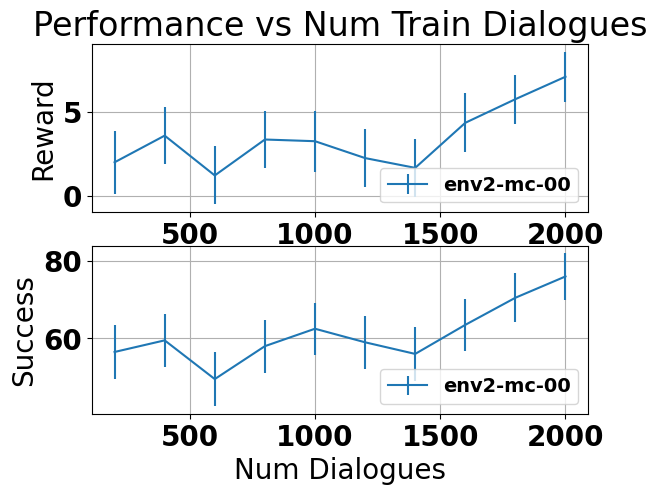
\includegraphics[width=\linewidth]{env2-CamRestaurants-mc.png}
      \caption{Monte-Carlo}
      \label{fig:mc}
    \endminipage
\end{figure}

\subsection{Chatting with a Q-network}
Here are presented examples of dialogs conducted with a Q-network. System sometimes gets caught in the loop and keeps asking the same question. The reason might be that semantic decoder didn't work well and haven't recog\-nised an input correctly, so the system continues to request more information. TODO get example

There was no instances in the dataset where the user wouldn't care which price range is there, and the dialog is ruined when this case is encountered (Dialog \ref{diag:with-price} vs Dialog \ref{diag:without-price}). This might happen due to insufficient semantic decoder knowledge and not enough of such samples in the database.

\begin{figure}[!htb]
    \minipage{0.49\textwidth}
      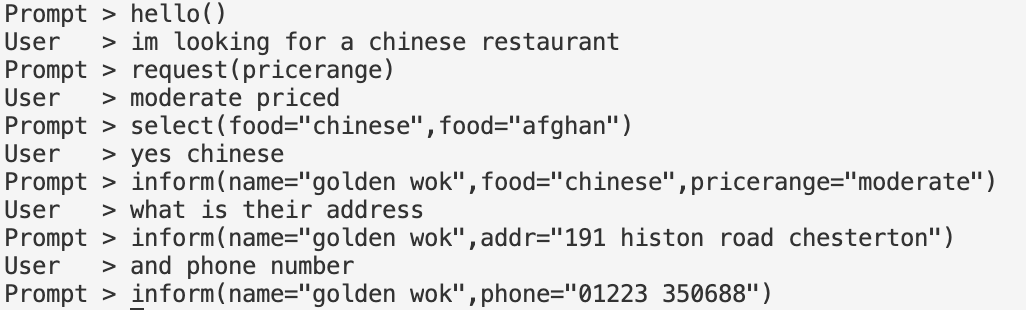
\includegraphics[width=\linewidth]{with_price.png}
      \caption{}
      \label{diag:with-price}
    \endminipage\hfill
    \minipage{0.49\textwidth}%
      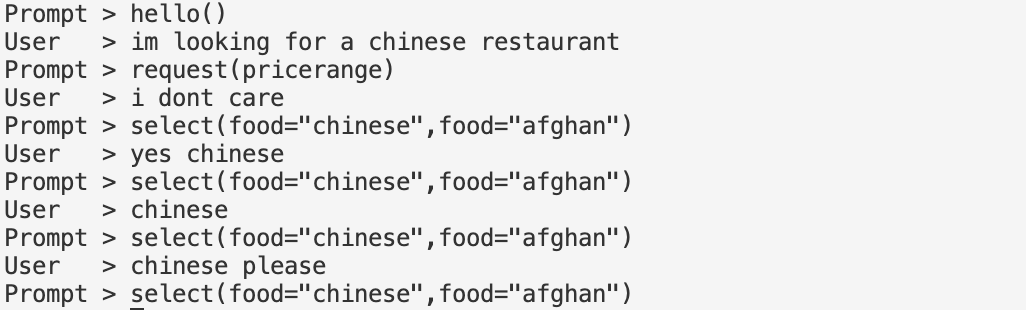
\includegraphics[width=\linewidth]{without_price.png}
      \caption{}
      \label{diag:without-price}
    \endminipage
\end{figure}

Examples with negations are performing poorly, most probably the failure of the semantic decoder not recognizing negation and not enough of negative samples in the database (Dialog \ref{diag:negation}).

\begin{figure}
    \centering
    \includegraphics[width=5cm]{chinese\ negation.png}
    \caption{}
    \label{diag:negation}
\end{figure}

\pagebreak

\section{Information Gain}

One can also substitute overall reward $r$ with $r = r + \nu r_i$, here $r_i$ is an additional intrinsic reward, and $\nu$ is a hyperparameter. This reward is called information gain and it measures how much additional information the system gets about user needs after one turn. Let action be of form $\{request, confirm,$ $select\}\_\xi$, $p_{\xi}$ and ${p_{\xi}}^\prime$ --- belief distributions over possible values of $\xi$ in current and next belief state.  Informa\-tion gain then is the distance between these distributions measured by with Jensen-Shannon di\-vergence distance:

\begin{equation}
    r_i(s, a, s\prime) =
    \begin{cases}
        d(p_{\xi}, p_{\xi}^\prime) \\
        0, \text{if } a \notin \text{\{request, confirm, select\}}
    \end{cases}
\end{equation}
where
\begin{equation}
    \begin{aligned}
        &d(p, q) = JS(p,q) = \frac{1}{2}(KL[p||m] + KL[q||m]), \\
        &m = \frac{1}{2}(p + q)
    \end{aligned}
\end{equation}

When distance is big enough (higher than a threshold) we add infor\-mation gain to the reward, but only when the action was of the form $\{request,$ $ confirm, select\}$. Intuitively it also doesn't make sense to calculate infor\-mation gain for actions like $bye, inform$ as they do not provide any additonal infor\-mation on user needs and therefore do not lead to the accomplishment of the dialog goal. It is beneficial to use intrinsic rewards in addition as they encourage system to get more useful information from users by requesting more from them, selecting the most relevant one information and confirming the choices.

Here one can see the difference in training with information gain and without it. Information gain improves the speed of training and slightly improves an overall performance from $96\%$  to $98.4\%$ (see Figure 7, 8).

\begin{figure}[!htb]
    \minipage{0.5\textwidth}
      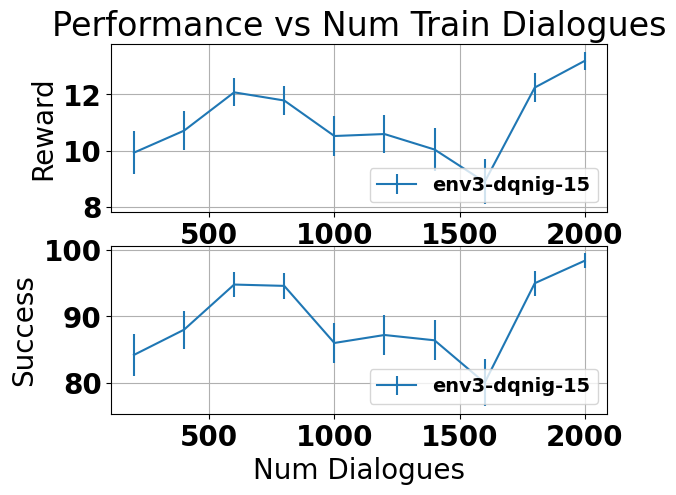
\includegraphics[width=\linewidth]{env3-ig-CamRestaurants.png}
      \caption{Information Gain}
    \endminipage\hfill
    \minipage{0.5\textwidth}
      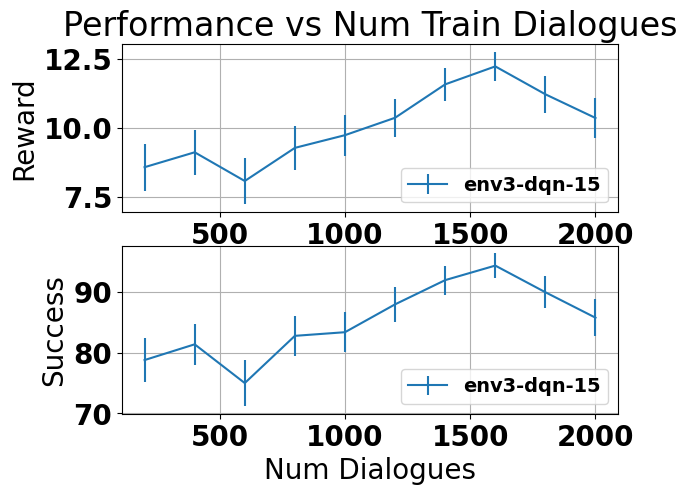
\includegraphics[width=\linewidth]{env3-CamRestaurants.png}
      \caption{No Information Gain}
    \endminipage
\end{figure}

One can also substitute $r = r + \nu r_i$. However one should be cautious --- if the value $\mu$ is too high, we push the sytem to gather more and more information and discourage it from making a choice and informing a user about it. 

\pagebreak

\section{Conclusion}
This report gives a brief introduction to the construction of spoken dialog systems. It contains research on different approaches and algorithms used for end-to-end spoken dialog system, that are build via modular approach. Such system was built with the use of different deep learning approaches, all approaches for each of the modules were studied and compared, several dialogs were conducted with the system. The results of the study were described and presented.

\pagebreak
\begin{thebibliography}{ccccc}
\addcontentsline{toc}{section}{Literatur}

%So kann eine eine Monographie zitieren:
\bibitem{Arbarello et al 1985}
E.\ Arbarello, M.\ Cornalba, P.\ Griffiths, J.\ Harris:
Geometry of algebraic curves. I. 
Springer, New York, 1985.

%So kann man eine Originalarbeit zitieren:
\bibitem{Shepherd-Barron 1997}
N.\ Shepherd-Barron:
Fano threefolds in positive characteristic.
Compositio Math.\  105  (1997),  237--265.

\end{thebibliography}
\end{document}